\chapter{Evaluation} % Main chapter title

\label{Chapter6} % Change X to a consecutive number; for referencing this chapter elsewhere, use \ref{ChapterX}


\section{Testing Methodology}

In order to ensure that the data collected for analysis is accurate and directly comparable, the testing environment must be kept exactly the same between trials and between different applications.
This gives each application the exact same starting conditions, and the best chance to demonstrate it's unabated performance.
For these tests, the host machine is a desktop computer running Windows 10 with a AMD Ryzen 9 5900X CPU and a Nvidia RTX 3070 GPU running the latest GeForce Experience version \emph{3.25.0.84}.
This configuration does not change throughout testing.
The client machine is the CM4 board attached to the PCB developed in Chapter \ref{Chapter4}, running the custom Manjaro linux distribution and forked version of Moonlight developed in Chapter \ref{Chapter5}.
This configuration also does not change throughout testing.
Each test is performed with both the host computer and the client machine running on the same network, with both devices connected to the same router using an ethernet cable.
This ensures that the speed of the network is not a factor in the tests.
The tests are performed multiple times under the following conditions:

\begin{itemize}
  \item Ideal Conditions: No other applications are running during testing.
  \item CPU Stressed: The CPU is constantly at 100\% load during the entire test.
  \item GPU Stressed: The GPU is constantly at 100\% load during the entire test.
\end{itemize}

\noindent
For each test, the following steps are performed:

\begin{enumerate}
  \item Both the host and client computers are fully rebooted to ensure no other application is running.
  \item The host computer starts up a single browser window with the web page described in Section \ref{sec:DevelopingTestingAndMeasurementTools}.
  \item If the test calls for the CPU or the GPU to be stressed, the application \enquote{Blender} is started on the host machine, and a benchmark is performed for the CPU or the GPU.
        This benchmark will run for longer than the duration of the test, and will keep the CPU or GPU at 100\% load for the entire duration of the benchmark.
  \item Both devices start up their respective data collection tool that will record key-strokes and changes in the screen's color.
  \item The client machine connects to the host computer using the application being tested.
  \item The user presses the \enquote{0} key on the client's numpad to synchronize the two devices' data recording tools.
  \item The user begins by typing on the client's keyboard slowly, allowing both computers to record their data.
  \item The user then types on the client's keyboard quickly to ensure that quick successive inputs are handled correctly and no data is lost or duplicated.
  \item Once typing is complete, both the client and the host computers close their data recording tools and the client ends the streaming session.
\end{enumerate}

\noindent
This process is repeated for each of the following applications:

\begin{itemize}
  \item The forked version of Moonlight developed for this project.
  \item Chrome Remote Desktop (CRD, Section \ref{subsec:ChromeRemoteDesktop}).
  \item Microsoft's Remote Desktop Connection (RDP, Section \ref{subsec:RemoteDesktopProtocol}).
  \item Virtual Network Computing (VNC, Section \ref{subsec:VirtualNetworkComputing}).
\end{itemize}

\noindent
Once all the data is collected, the data from the host and client machines for a single trial are organized into a single CSV file for processing.
In order to ensure that the data is comparable, all extraneous factors must be removed from the data.
Namely, the network latency and difference in computer clocks must be removed.
This is partially accounted for in step \emph{6} of the above process, and the remaining inaccuracy can now be removed by subtracting the time difference between the when the client presses the button and the time the host executes that command.
This ensures that any inaccuracies in each computer's internal clock will not impact the data.

After the data is cleaned up, the data can be processed by matching each key-stroke and change in the screen's color detected by the client and host machines and calculating how much time elapsed between the events.
This reveals the amount of delay the user experiences between when they press a key and when the host executes the command, and between when they press a key and can visually see the response.


\section{Responsivity and Latency}

\todosection

\begin{figure}[h]
  \centering
  \begin{tikzpicture}
    \begin{axis}[
      boxplot/draw direction=y,
      ylabel={Time (ms)},
      scale only axis,
      height=8cm,
      width=\textwidth,
      ymin=0,ymax=200,
      cycle list={{black},{blue},{red}},
      legend style={
          legend pos=outer north east,
          font=\small
        },
      legend cell align=left,
      legend image code/.code={%
          \draw[#1] (0cm,-0.1cm) rectangle (0.6cm,0.1cm);
        },
      boxplot={
          % Three boxplots for each column
          draw position={1/4 + floor(\plotnumofactualtype/3) + 1/4*mod(\plotnumofactualtype,3)},
          % Each plot takes up a quarter of the column
          box extend=0.2,
        },
      % 1 unit in x controls the width:
      x=2cm,
      % ... and it means that we should describe intervals:
      xtick={0,1,2,...,10},
      x tick label as interval,
      xticklabels={%
      {Forked Moonlight\\{\tiny ideal/cpu/gpu}},%
      {CRD\\{\tiny ideal/cpu/gpu}},%
      {RDP\\{\tiny ideal/cpu/gpu}},%
      {VNC\\{\tiny ideal/cpu/gpu}},%
      },
      x tick label style={
          text width=2.5cm,
          align=center
        },
      ]

      % Forked Moonlight
      \addplot
      table[col sep=comma,x=Time difference] {Data/ideal/moonlight_key_delay.csv};
      \addplot
      table[col sep=comma,x=Time difference] {Data/stresscpu/moonlight_key_delay.csv};
      \addplot
      table[col sep=comma,x=Time difference] {Data/stressgpu/moonlight_key_delay.csv};

      % CRD
      \addplot
      table[col sep=comma,x=Time difference] {Data/ideal/crd_key_delay.csv};
      \addplot
      table[col sep=comma,x=Time difference] {Data/stresscpu/crd_key_delay.csv};
      \addplot
      table[col sep=comma,x=Time difference] {Data/stressgpu/crd_key_delay.csv};

      % RDP
      \addplot
      table[col sep=comma,x=Time difference] {Data/ideal/rdp_key_delay.csv};
      \addplot
      table[col sep=comma,x=Time difference] {Data/stresscpu/rdp_key_delay.csv};
      \addplot
      table[col sep=comma,x=Time difference] {Data/stressgpu/rdp_key_delay.csv};

      % VNC
      \addplot
      table[col sep=comma,x=Time difference] {Data/ideal/vnc_key_delay.csv};
      \addplot
      table[col sep=comma,x=Time difference] {Data/stresscpu/vnc_key_delay.csv};
      \addplot
      table[col sep=comma,x=Time difference] {Data/stressgpu/vnc_key_delay.csv};

      \legend{Ideal,CPU stressed,GPU stressed}
    \end{axis}
  \end{tikzpicture}
  \caption[Input Delay Data]{Time for host to press key from client.}
  \label{fig:InputDelay}
\end{figure}

\begin{figure}[h]
  \centering
  \begin{tikzpicture}
    \begin{axis}[
      boxplot/draw direction=y,
      ylabel={Time (ms)},
      scale only axis,
      height=8cm,
      width=\textwidth,
      ymin=0,ymax=200,
      cycle list={{black},{blue},{red}},
      legend style={
          legend pos=outer north east,
          font=\small
        },
      legend cell align=left,
      legend image code/.code={%
          \draw[#1] (0cm,-0.1cm) rectangle (0.6cm,0.1cm);
        },
      boxplot={
          % Three boxplots for each column
          draw position={1/4 + floor(\plotnumofactualtype/3) + 1/4*mod(\plotnumofactualtype,3)},
          % Each plot takes up a quarter of the column
          box extend=0.2,
        },
      % 1 unit in x controls the width:
      x=2cm,
      % ... and it means that we should describe intervals:
      xtick={0,1,2,...,10},
      x tick label as interval,
      xticklabels={%
      {Forked Moonlight\\{\tiny ideal/cpu/gpu}},%
      {CRD\\{\tiny ideal/cpu/gpu}},%
      {RDP\\{\tiny ideal/cpu/gpu}},%
      {VNC\\{\tiny ideal/cpu/gpu}},%
      },
      x tick label style={
          text width=2.5cm,
          align=center
        },
      ]

      % Forked Moonlight
      \addplot
      table[col sep=comma,x=Time difference] {Data/ideal/moonlight_color_delay.csv};
      \addplot
      table[col sep=comma,x=Time difference] {Data/stresscpu/moonlight_color_delay.csv};
      \addplot
      table[col sep=comma,x=Time difference] {Data/stressgpu/moonlight_color_delay.csv};

      % CRD
      \addplot
      table[col sep=comma,x=Time difference] {Data/ideal/crd_color_delay.csv};
      \addplot
      table[col sep=comma,x=Time difference] {Data/stresscpu/crd_color_delay.csv};
      \addplot
      table[col sep=comma,x=Time difference] {Data/stressgpu/crd_color_delay.csv};

      % RDP
      \addplot
      table[col sep=comma,x=Time difference] {Data/ideal/rdp_color_delay.csv};
      \addplot
      table[col sep=comma,x=Time difference] {Data/stresscpu/rdp_color_delay.csv};
      \addplot
      table[col sep=comma,x=Time difference] {Data/stressgpu/rdp_color_delay.csv};

      % VNC
      \addplot
      table[col sep=comma,x=Time difference] {Data/ideal/vnc_color_delay.csv};
      \addplot
      table[col sep=comma,x=Time difference] {Data/stresscpu/vnc_color_delay.csv};
      \addplot
      table[col sep=comma,x=Time difference] {Data/stressgpu/vnc_color_delay.csv};

      \legend{Ideal,CPU stressed,GPU stressed}
    \end{axis}
  \end{tikzpicture}
  \caption[Color Delay Data]{Time for client to receive update to screen.}
  \label{fig:ColorDelay}
\end{figure}

\begin{figure}[h]
  \centering
  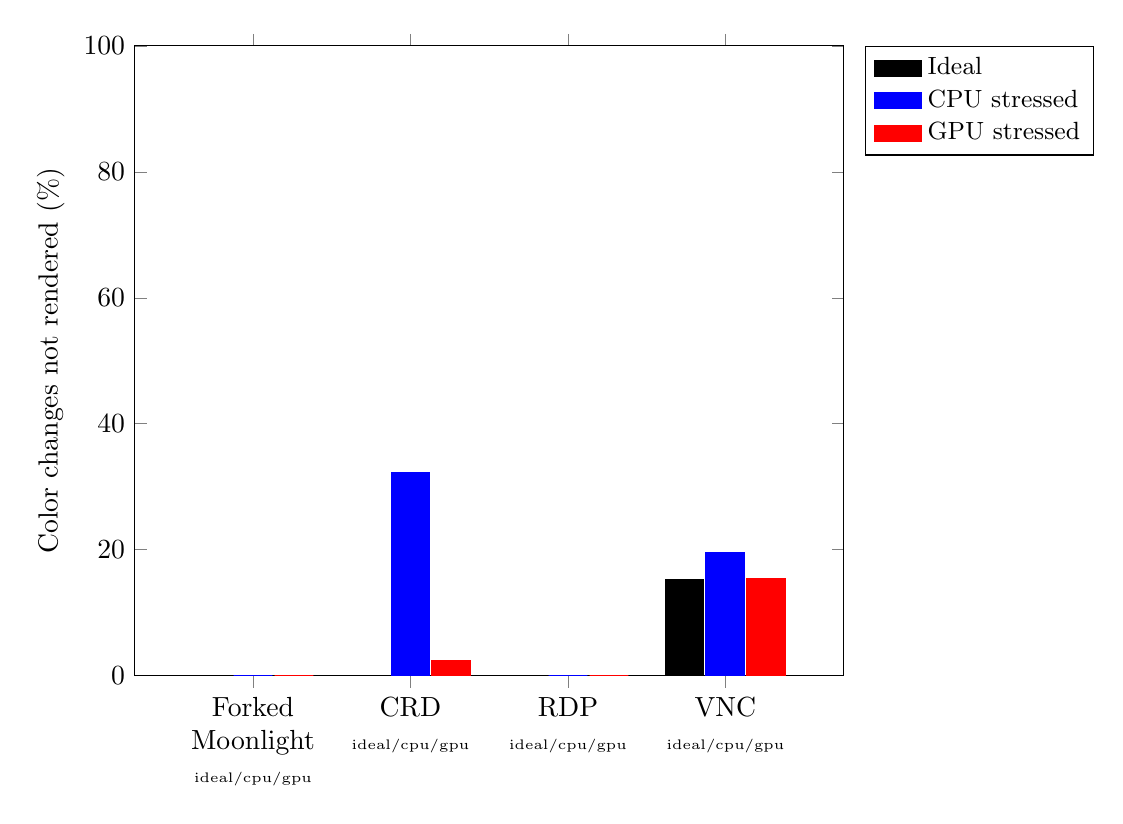
\begin{tikzpicture}
    \begin{axis}[
      ylabel={Color changes not rendered (\%)},
      scale only axis,
      height=8cm,
      width=\textwidth,
      enlarge x limits=0.25,
      ybar=2*\pgflinewidth,
      bar width=14pt,
      ymin=0,ymax=100,
      cycle list={{black},{blue},{red}},
      legend style={
          legend pos=outer north east,
          font=\small
        },
      legend cell align=left,
      legend image code/.code={%
          \draw[#1] (0cm,-0.1cm) rectangle (0.6cm,0.1cm);
        },
      % 1 unit in x controls the width:
      x=2cm,
      % ... and it means that we should describe intervals:
      xtick={0,1,2,...,10},
      % x tick label as interval,
      xticklabels={%
      {Forked Moonlight\\{\tiny ideal/cpu/gpu}},%
      {CRD\\{\tiny ideal/cpu/gpu}},%
      {RDP\\{\tiny ideal/cpu/gpu}},%
      {VNC\\{\tiny ideal/cpu/gpu}},%
      },
      x tick label style={
          text width=2.5cm,
          align=center
        },
      ]
      \addplot[style={black,fill=black,mark=none}]
      coordinates {(0, 0) (1,0) (2,0) (3,15.32)};

      \addplot[style={blue,fill=blue,mark=none}]
      coordinates {(0,0) (1,32.28) (2,0) (3,19.51)};

      \addplot[style={red,fill=red,mark=none}]
      coordinates {(0,0) (1,2.34) (2,0) (3,15.5)};

      \legend{Ideal,CPU stressed,GPU stressed}
    \end{axis}
  \end{tikzpicture}
  \caption[Color Delay Loss Data]{Percentage of color changes not rendered.}
  \label{fig:ColorDelayLoss}
\end{figure}


\section{Performance}

\todosection


\section{Quality}

\todosection


\section{Summary}

\todosection